% !TeX encoding = UTF-8
% !TeX program = xelatex
\documentclass[12pt,a4paper]{article}
\usepackage{xeCJK} % 须放在\usepackage{}列中足够前的位置
\usepackage{fontspec}
\usepackage{graphicx}
\usepackage{caption}
\usepackage{enumerate}
\usepackage{setspace}
\usepackage{array} % 製作表格必須的宏包
\usepackage{tabularx} % 自動調整列寬的表格宏包
\usepackage{adjustbox}
\usepackage{listings}
\usepackage{caption}
\usepackage{xcolor}
\usepackage{longtable} 
\usepackage{hyperref} 
\setCJKfamilyfont{heiti}{Heiti TC}
\CJKfamily{heiti}
\setmainfont{Arial}
\setstretch{1.5}
\usepackage{geometry}

% 調整頁面邊距
\geometry{
    top=2cm,          % 縮小上邊距
    bottom=2cm,
    left=2cm,
    right=2cm
}

% 調整標題間距
\usepackage{titling}
\setlength{\droptitle}{-4em}    % 減少標題前的空白
\pretitle{\begin{center}\Large\bfseries}
\posttitle{\par\end{center}}
\preauthor{\begin{center}
    \large}
\postauthor{\end{center}}
\predate{\begin{center}\large}
\postdate{\par\end{center}}


% 程式碼區塊的樣式設置
\lstset{
    language=C,
    basicstyle=\ttfamily\small,
    numbers=left,
    numberstyle=\tiny,
    frame=single,
    breaklines=true,
    keywordstyle=\color{blue},
    commentstyle=\color{green!60!black},
    stringstyle=\color{red},
    showstringspaces=false,
    tabsize=4,
    inputencoding=utf8  % 添加這行
}


\begin{document}

\title{1131 數位影像處理 HW 02}
\author{資訊三甲 \quad D1109023 \quad 楊孟憲}
\date{}
\maketitle

\section*{摘要}
此次作業實作分為兩個部分;第一部分需要讀取照片後取得顏色的直方圖(Histogram),第二部分則是運算獲得直方圖均化 (Histogram Equalization) 以及生成直方圖均化後的結果。\\[5pt]
\textbf{完整程式碼:}
\href{https://github.com/mengxian0913/FCU_Image_Process_Record/blob/master/lab02/app.cpp}{Link to github}

\section{開發環境以及工具}
    \begin{itemize}
        \item 開發環境:macOS
        \item 程式語言:C++
        \item 編譯版本:clang++ -std=c++17
        \item 下載 openCV4
    \end{itemize}

\section{專案目錄}
\begin{minipage}{\textwidth} 
    \begin{tabular}{ll}
        \texttt{./images/*} & 準備好兩組照片 \\
        \texttt{./res/*} & 圖片輸出結果 \\
        \texttt{app.cpp} & 主程式 \\
        \texttt{./a.out} & 執行檔案 \\
    \end{tabular}
\end{minipage}


% 这里需要插入图片
% \includegraphics[width=0.8\textwidth]{name_image.jpg}


\section{直方圖(Histogram)}
\begin{minipage}{\textwidth} 
    實作讀取圖片後,分析顏色的 B, G, R 的分佈,並生成直方圖。(0 $\sim$ 255) \\
    這邊實作是以預設為三個通道的方式來做實作。以下講解彩色、灰階以及黑白的不同。
    \begin{itemize}
        \item 彩色:B, G, R 通道值可能不一樣( 介於 0 ~ 255 之間)。
        \item 灰階:B, G, R 通道的值必須一樣( 介於 0 ~ 255 之間)。
        \item 黑白:B, G, R 通道的值必須一樣( 只能為兩個數值,通常設定為 0 和 255 )
    \end{itemize}
    PS1.因為避免在像素很多的時候有顏色偏差導致直方圖某些值變太高,不易展示和閱覽,所以會將圖片大小控制在一定的範圍中。我會先手動將圖片寬度訂在 200px。 \\[1.4pt]
    PS1.不管彩色或是黑白,輸出的直方圖都是三張,如果是黑白,就是輸出三張長得一樣的圖直方圖。
\end{minipage}


\subsection{結果展示}
\begin{center}
\begin{longtable}{|c|c|c|c|c|}
\hline
Channel/Image & Origin & B & G & R \\
\hline
\endfirsthead

\hline
Channel/Image & Origin & B & G & R \\
\hline
\endhead

Tiger & 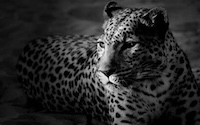
\includegraphics[width=0.2\textwidth]{./latexSource/tiger_origin.png} & 
       
\includegraphics[width=0.2\textwidth]{./latexSource/tiger_B_HIS.png} & 
       
\includegraphics[width=0.2\textwidth]{./latexSource/tiger_G_HIS.png} & 
       
\includegraphics[width=0.2\textwidth]{./latexSource/tiger_R_HIS.png} \\
\hline
Woman & 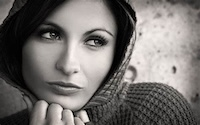
\includegraphics[width=0.2\textwidth]{./latexSource/woman_origin.png} & 
       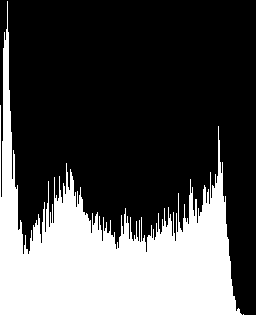
\includegraphics[width=0.2\textwidth]{./latexSource/woman_B_HIS.png} & 
       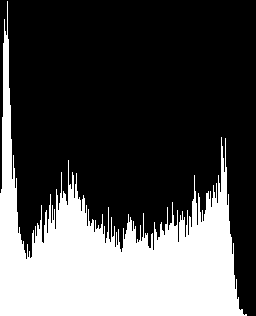
\includegraphics[width=0.2\textwidth]{./latexSource/woman_G_HIS.png} & 
       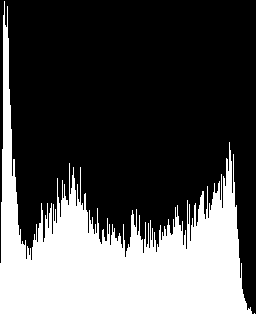
\includegraphics[width=0.2\textwidth]{./latexSource/woman_R_HIS.png} \\
\hline
Dog & 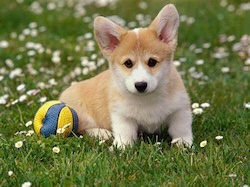
\includegraphics[width=0.2\textwidth]{./latexSource/dog_origin.png} & 
       
\includegraphics[width=0.2\textwidth]{./latexSource/dog_B_HIS.png} & 
       
\includegraphics[width=0.2\textwidth]{./latexSource/dog_G_HIS.png} & 
       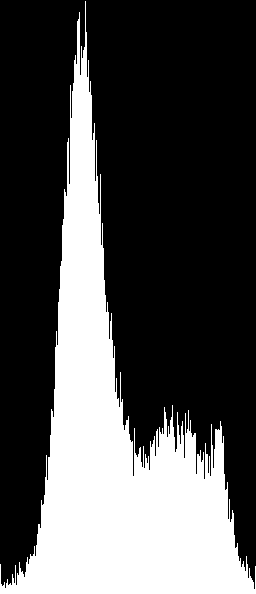
\includegraphics[width=0.2\textwidth]{./latexSource/dog_R_HIS.png} \\ 
\hline
Canada & 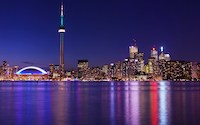
\includegraphics[width=0.2\textwidth]{./latexSource/Canada_origin.png} & 
       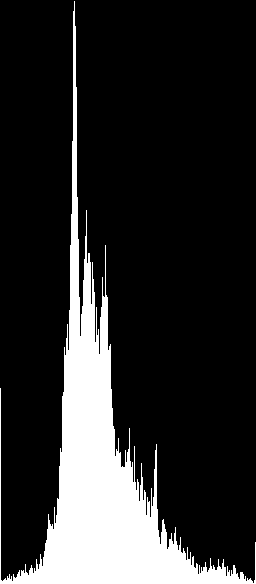
\includegraphics[width=0.2\textwidth]{./latexSource/Canada_B_HIS.png} & 
       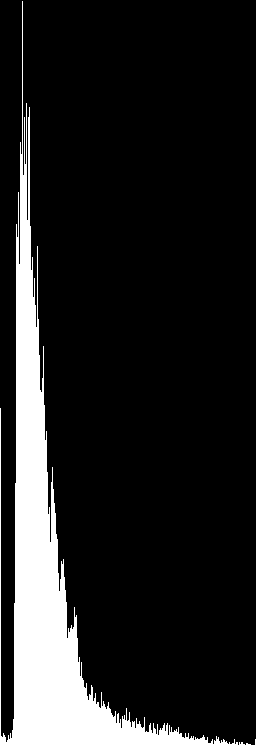
\includegraphics[width=0.2\textwidth]{./latexSource/Canada_G_HIS.png} & 
       
\includegraphics[width=0.2\textwidth]{./latexSource/Canada_R_HIS.png} \\ 
\hline
\end{longtable}
\end{center}



\subsection{實作代碼及註解}
實作一個 struct ,其中包含了原始圖片、均化後的圖片、均化前的直方圖(B, G, R)、均化後的直方圖(B, G, R),以及圖片的寬高。
另外使用 C++ 內建的 STL 工具,創建直方圖(均前 / 後)的 mapping 關係,key 代表顏色強度;value 代表出現的個數。\\
另外創建一個 vector 用來記錄前綴和。

\lstinputlisting[caption={Image struct and Histogram generation}]{./latexSource/sourceCode/a.cpp}


\section{直方圖均化 (Histogram Equalization)}
將直方圖均化的意義就是避免差值過大,所以用分佈的概念來均攤個強度出現的次數。實作方法很簡單,使用前綴和計算當下狀態的分佈狀況後,再重新分布。 \\
為了保持程式結構清晰,將均化前後的映射表(map)分開宣告,這樣可以直接進行像素值的轉換,提高程式的可讀性和效能。 \\

\textbf{計算公式如下:}

\[
newValue = value  \times \frac{subSum}{totalSum}
\]


\begin{center}
    \begin{longtable}{|c|c|c|c|c|}
    \hline
    Channel/Image & Origin & B & G & R \\
    \hline
    \endfirsthead
    
    \hline
    Channel/Image & Origin & B & G & R \\
    \hline
    \endhead
    
    Tiger & 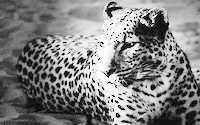
\includegraphics[width=0.2\textwidth]{./latexSource/tiger_process.png} & 
           
\includegraphics[width=0.2\textwidth]{./latexSource/tiger_B_EQUA.png} & 
           
\includegraphics[width=0.2\textwidth]{./latexSource/tiger_G_EQUA.png} & 
           
\includegraphics[width=0.2\textwidth]{./latexSource/tiger_R_EQUA.png} \\
    \hline
    Woman & 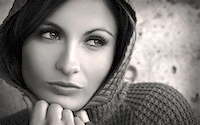
\includegraphics[width=0.2\textwidth]{./latexSource/woman_process.png} & 
           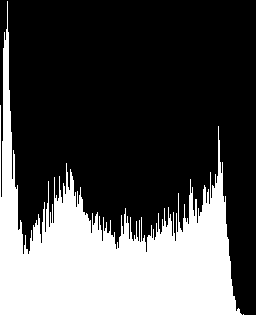
\includegraphics[width=0.2\textwidth]{./latexSource/woman_B_EQUA.png} & 
           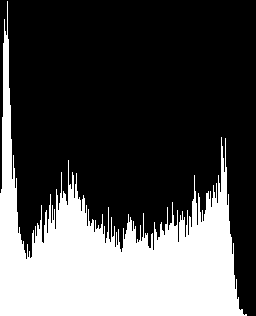
\includegraphics[width=0.2\textwidth]{./latexSource/woman_G_EQUA.png} & 
           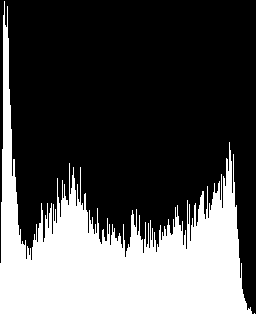
\includegraphics[width=0.2\textwidth]{./latexSource/woman_R_EQUA.png} \\
    \hline
    Dog & 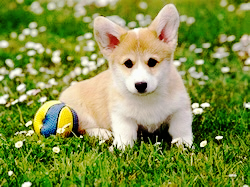
\includegraphics[width=0.2\textwidth]{./latexSource/dog_process.png} & 
           
\includegraphics[width=0.2\textwidth]{./latexSource/dog_B_EQUA.png} & 
           
\includegraphics[width=0.2\textwidth]{./latexSource/dog_G_EQUA.png} & 
           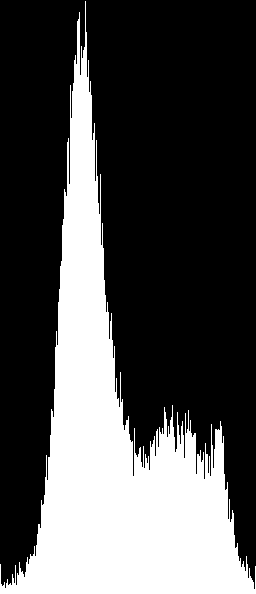
\includegraphics[width=0.2\textwidth]{./latexSource/dog_R_EQUA.png} \\ 
    \hline
    Canada & 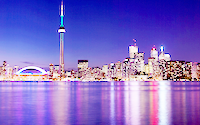
\includegraphics[width=0.2\textwidth]{./latexSource/Canada_process.png} & 
           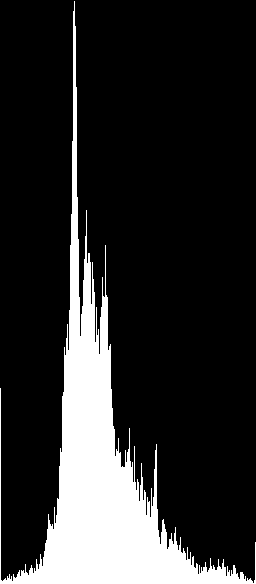
\includegraphics[width=0.2\textwidth]{./latexSource/Canada_B_EQUA.png} & 
           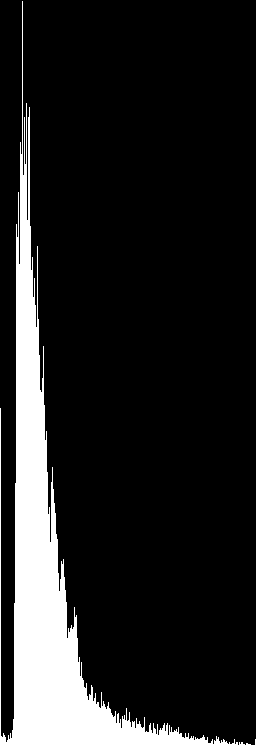
\includegraphics[width=0.2\textwidth]{./latexSource/Canada_G_EQUA.png} & 
           
\includegraphics[width=0.2\textwidth]{./latexSource/Canada_R_EQUA.png} \\ 
    \hline
    \end{longtable}
    \end{center}
    
\subsection{實作代碼及註解}

\lstinputlisting[caption={Histogram Equalization}]{./latexSource/sourceCode/b.cpp}

\section{前後對比圖}

\begin{center}
    \begin{longtable}{|c|c|c|}
    \hline
        Compare/Image & Origin & Process \\
    \hline
    \endfirsthead
    
    \hline
        Compare/Image & Origin & Process \\
    \hline
    \endhead
    
    Tiger & 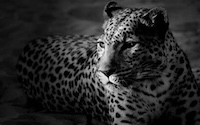
\includegraphics[width=0.2\textwidth]{./latexSource/tiger_origin.png} & 
           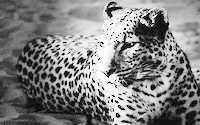
\includegraphics[width=0.2\textwidth]{./latexSource/tiger_process.png} \\
    \hline
    Woman & 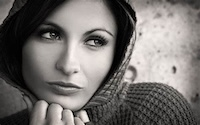
\includegraphics[width=0.2\textwidth]{./latexSource/woman_origin.png} &
           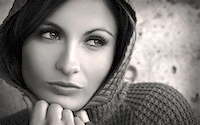
\includegraphics[width=0.2\textwidth]{./latexSource/woman_process.png} \\
    \hline
    Dog & 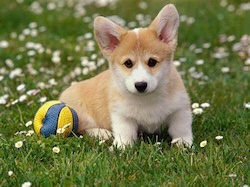
\includegraphics[width=0.2\textwidth]{./latexSource/dog_origin.png} & 
           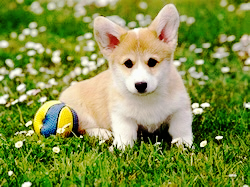
\includegraphics[width=0.2\textwidth]{./latexSource/dog_process.png} \\ 
    \hline
    Canada & 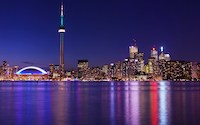
\includegraphics[width=0.2\textwidth]{./latexSource/Canada_origin.png} & 
           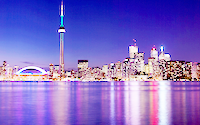
\includegraphics[width=0.2\textwidth]{./latexSource/Canada_process.png} \\ 
    \hline
    \end{longtable}
 \end{center}


\section{心得}

這次的直方圖均化作業讓我深入理解了數位影像處理中的幾個重要概念:

\begin{itemize}
    \item 掌握了影像直方圖的分析方法,包括 RGB 三個色彩通道的分布特性
    \item 理解了直方圖均化的原理,學會運用累積分布函數(CDF)來改善影像對比度
    \item 實作過程中對 OpenCV 的操作更加熟悉,特別是在矩陣運算和色彩空間轉換方面
    \item 透過觀察均化前後的結果,更加理解影像增強技術對視覺效果的影響
\end{itemize}

在實作過程中,雖然遇到了一些技術細節需要克服,像是圖片資訊過大導致直方圖難以閱讀以及如確保均化後的像素值正確映射到 [0,255] 範圍,但通過查詢資料和反覆驗證,最終都順利解決了這些問題。這次作業不僅強化了程式實作能力,也加深了對影像處理理論的認識。 \\

\end{document}
